\documentclass[12pt,a4paper,openright,twoside]{book}
\usepackage[utf8]{inputenc}
\usepackage{disi-thesis}
\usepackage{code-lstlistings}
\usepackage{notes}
\usepackage{shortcuts}
\usepackage{acronym}

\school{\unibo}
\programme{Corso di Laurea in Ingegneria e Scienze Informatiche}
\title{Servizio di diagnostica della latenza in una rete anycast}
\author{Foschi Gioele}
\date{\today}
\subject{Programmazione ad Oggetti}
\supervisor{Prof. Mirko Viroli}
\cosupervisor{Francesco Collini}
\morecosupervisor{Stefano Babini}
\session{I}
\academicyear{2025-2026}

% Definition of acronyms
\acrodef{DNS}{Domain Name Server}
\acrodef{BGP}{Border Gateway Protocol}
\acrodef{IP}{Internet Protocol}
\acrodef{HTTP}{Hypertext Transfer Protocol}

\mainlinespacing{1.241} % line spacing in mainmatter, comment to default (1)

\begin{document}

\frontmatter\frontispiece

\begin{abstract}	
Il progetto è incentrato sulla modernizzazione architetturale e sul re-engineering dei 
servizi di misurazione della latenza in una rete anycast. Il sistema preesistente, 
basato su architettura PHP/Apache e script di fan-out Python, soffriva di limitazioni 
prestazionali, elevato overhead di CPU/memoria, una bassa affidabilità di risposta ed eccessiva rigidità nella gestione dell'I/O concorrente.

Il progetto ha coinvolto la riscrittura di due sotto-servizi principali. Il servizio di 
downstream, incaricato di calcolare la latenza tra il server stesso e la macchina 
specificata in input, era originariamente scritto in PHP ed è stato riprogettato in Go, 
adottando i principi della Clean Architecture e un design basato su design pattern, massimizzando l'affidabilità della risposta. Il servizio di upstream, responsabile dell'aggregazione dei dati raccolti dalle interrogazioni dei server di downstream, era originariamente scritto in Python ed è stato anch'esso riscritto in Go, sfruttando il modello di concorrenza nativo del linguaggio (goroutine e channel) per superare la rigidità nella gestione dell'I/O concorrente riscontrata nel sistema preesistente.

Il nuovo sistema è stato validato confrontandolo con l'architettura preesistente,
mostrando un miglioramento dell'affidabilità del servizio e una riduzione dell'utilizzo 
di memoria sui server di dispiegamento. Il lavoro ha incluso inoltre la progettazione 
di un'interfaccia utente modernizzata per il nuovo applicativo.
\end{abstract}

\begin{dedication} % this is optional
Optional. Max a few lines.
\end{dedication}

%----------------------------------------------------------------------------------------
\tableofcontents   
\listoffigures
\lstlistoflistings
%----------------------------------------------------------------------------------------

\mainmatter
\chapter{Introduzione}
\label{chap:introduction}

Il presente documento descrive le attività svolte durante il periodo di tirocinio aziendale presso FlashStart, sotto la supervisione del Prof. Mirko Viroli, i tutor aziendali Francesco Collini e Stefano Babini.

FlashStart è una azienda che da oltre 20 anni protegge gli utenti nel mondo digitale con soluzioni di sicurezza informatica attraverso il filtraggio dei contenuti basato su \ac{DNS} e intelligenza artificiale.
L'azienda fornisce filtraggio dei contenuti per utenti singoli e organizzazioni di ogni dimensione.
FlashStart opera su una rete anycast\footnote{Anycast è una metodologia di indirizzamento di rete dove le richieste vengono indirizzate ad una varietà di diversi nodi. Tipicamente si indirizza il traffico in entrata al server più vicino che ha la capacità di processare la richiesta efficientemente.} globale composta da più di 160 nodi distribuiti strategicamente in tutti i continenti, progettata per garantire elevata disponibilità, latenza minima e continuità operativa anche in caso di interruzioni o picchi di traffico.

A partire dal 2026 FlashStart ha iniziato il più grande redesign dell'azienda, spostandosi da una applicazione con architettura monolitica ad un applicativo moderno con una architettura basata su microservizi altamente scalabili.
In questo documento si farà riferimento ai due applicativi come: \textit{FlashStart Cloud}, il sistema attualmente in uso ma destinato alla dismissione, e \textit{FlashStart Internet Protection 2026}, la soluzione individuata per la sua sostituzione.

Nel seguito della trattazione, per semplicità, si farà riferimento al nuovo sistema come \textit{FlashStart 2026}.

\paragraph{Contributo della tesi}
Lo strumento di controllo della latenza rappresenta un strumento fondamentale nel toolkit del Network Admin, poiché consente di stimare a priori il tempo di risposta del servizio \ac{DNS} (espresso in millisecondi) che l'utente finale sperimenterà nell'utilizzo del servizio di protezione della navigazione offerto da FlashStart. Questa stima preventiva permette di individuare eventuali criticità infrastrutturali prima che queste si traducano in un degrado percepibile dell'esperienza utente, fornendo così un supporto decisionale concreto per le attività di monitoraggio e ottimizzazione della rete.
Dal momento che la protezione erogata da FlashStart opera ``at \ac{DNS} levek'', una latenza contenuta, tipicamente inferiore ai $10 \text{ ms}$, risulta essenziale per coniugare due esigenze apparentemente in tensione tra loro: da un lato garantire un livello adeguato di sicurezza nella navigazione, dall'altro preservarne la fluidità, evitando che l'utente percepisca rallentamenti o ritardi nella risoluzione dei nomi di dominio. Un servizio di sicurezza percepito come ``lento'' rischia infatti di essere disabilitato o aggirato dagli utenti stessi, vanificando l'obiettivo protettivo per cui è stato progettato.
Oltre alla misurazione della latenza sul nodo preferenziale, lo strumento è in grado di stimare eventuali nodi alternativi disponibili in caso di malfunzionamento o interruzione di servizio (outage) del nodo primario, individuato secondo il criterio del best latency path. Questa capacità predittiva è resa possibile dall'architettura di rete sottostante, basata sul protocollo \ac{BGP} in configurazione Anycast: gli indirizzi \ac{IP} del servizio di \ac{DNS} sicuro vengono infatti annunciati contemporaneamente da ogni datacenter della rete distribuita. Ne consegue che, in presenza di una criticità sul nodo primario, il traffico dell'utente viene automaticamente e trasparentemente rediretto verso un nodo alternativo, garantendo la continuità della navigazione filtrata e protetta, seppur con un incremento marginale della latenza rispetto alla condizione ottimale.

Il contributo principale di questo lavoro di tesi consiste nella migrazione del servizio di misurazione della latenza dalla precedente implementazione, originariamente sviluppata utilizzando i linguaggi PhP e Python, verso una nuova piattaforma progettata secondo criteri architetturali più moderni, coerenti e strutturati. Tale processo di migrazione non si è tuttavia limitato a una semplice traduzione o riscrittura del codice preesistente in un nuovo linguaggio o framework: ha comportato, al contrario, una revisione approfondita e critica dell'architettura sottostante, con l'obiettivo esplicito di superare i limiti strutturali e funzionali riscontrati nella soluzione originaria.
In particolare, il lavoro dovrà conseguire un miglioramento significativo lungo tre direttrici fondamentali. La prima riguarda l'affidabilità del sistema, intesa come la capacità di garantire un funzionamento stabile, coerente e resiliente anche in condizioni di carico elevato o di traffico anomalo, minimizzando il rischio di malfunzionamenti o interruzioni del servizio. La seconda riguarda l'efficienza operativa, perseguita attraverso l'ottimizzazione dell'utilizzo delle risorse computazionali disponibili e la conseguente riduzione dei tempi di risposta del sistema, elemento particolarmente critico trattandosi di uno strumento di misurazione della latenza stessa. La terza direttrice, infine, concerne l'usabilità della piattaforma, considerata sia dal punto di vista degli utenti finali che interagiscono con lo strumento, sia da quello degli sviluppatori incaricati di mantenerlo, estenderlo e aggiornarlo nel tempo, garantendo così la sostenibilità del progetto anche in una prospettiva di lungo periodo.
\paragraph{Struttura dei Capitoli}

\begin{description}
    \item[\Cref{chap:background} -- Sfondo tecnologico e architettura:] introduce il contesto tecnologico di riferimento, fornendo una descrizione dettagliata dell'architettura del servizio e delle sue componenti fondamentali (\emph{upstream orchestrator}, \emph{downstream} e il punto d'ingresso su FlashStart Cloud). Una particolare attenzione è rivolta all'individuazione e all'analisi sistematica delle fragilità e delle criticità dell'infrastruttura esistente, che costituiscono il punto di partenza motivazionale per il lavoro svolto.
    
    \item[\Cref{chap:analysis} -- Requisiti ed obiettivi:] definisce in modo formale i requisiti e gli obiettivi del progetto, strutturando i vincoli funzionali e architetturali prescritti per ciascun elemento del sistema sulla base delle criticità emerse dall'analisi precedente.
    
    \item[\Cref{chap:design} -- Scelte di design:] illustra le decisioni architetturali e di progettazione adottate al fine di soddisfare i requisiti individuati, formalizzando e motivando le scelte strutturali effettuate.
    
    \item[\Cref{chap:development} -- Sviluppo:] affronta nel dettaglio la fase realizzativa, argomentando la selezione dei linguaggi di programmazione utilizzati e descrivendo lo sviluppo analitico delle varie componenti del sistema.
    
    \item[\Cref{chap:results} -- Validazione e test:] presenta le prove sperimentali e i test condotti sul campo al fine di verificare la correttezza, la robustezza e le prestazioni dei componenti realizzati. Approfondisce inoltre le strategie e le decisioni operative adottate per il dispiegamento (\emph{deployment}) e l'integrazione delle nuove componenti all'interno dell'infrastruttura di rete e del nuovo applicativo.
    
    \item[\Cref{chap:conclusion} -- Conclusioni:] raccoglie le considerazioni finali sui risultati conseguiti e traccia le possibili direttrici per gli sviluppi e i perfezionamenti futuri.
\end{description}
\chapter{Background}
\label{chap:background}
Il presente capitolo introduce il contesto tecnico e infrastrutturale all'interno del quale si colloca il lavoro di tesi. 
In particolare, viene descritta l'architettura legacy del servizio di misurazione della latenza attualmente in produzione, sviluppato per supportare le esigenze operative di \emph{FlashStart Cloud}.
La comprensione approfondita di tale architettura, delle sue componenti e delle interazioni tra di esse costituisce un prerequisito indispensabile per individuare i limiti del sistema esistente e per motivare le scelte progettuali presentate nei capitoli successivi.

Di seguito viene descritta nel dettaglio l'architettura a tre componenti --- Upstream Orchestrator, Downstream e route PHP --- che costituisce il punto di partenza dell'analisi condotta in questo lavoro.

Il servizio di misurazione della latenza (di seguito \emph{latency service}) adotta un'architettura distribuita a tre componenti disaccoppiati, ciascuno responsabile di una fase distinta del processo di raccolta, aggregazione ed esposizione dei dati.
Le componenti comunicano tra loro in sequenza tramite chiamate \ac{HTTP}, secondo un modello \emph{orchestrator--worker} ricorrente nei sistemi progettati per il monitoraggio distribuito di infrastrutture di rete su larga scala.
La Figura~\ref{fig:legacy-architecture} illustra schematicamente il flusso di comunicazione tra le tre componenti; di seguito ciascuna di esse viene descritta in dettaglio.

\section{Upstream Orchestrator}
\label{section:upstream-orchestrator}

L'\emph{Upstream Orchestrator} rappresenta il componente centrale del sistema ed è localizzato all'interno del server principale dell'infrastruttura. Le sue responsabilità principali sono le seguenti:

\begin{itemize}
    \item \emph{Discovery dei server attivi}: recupera dinamicamente la lista dei server della rete da interrogare ai fini della misurazione della latenza, garantendo che solo i nodi effettivamente operativi vengano coinvolti nel processo di raccolta;
    \item \emph{Distribuzione delle richieste}: inoltra, tramite chiamate \ac{HTTP}, le richieste di misurazione verso ciascun nodo Downstream individuato nella fase precedente;
    \item \emph{Aggregazione dei risultati}: raccoglie le risposte provenienti dai singoli nodi Downstream, effettuando l'unione dei dati parziali in un'unica struttura coerente;
    \item \emph{Riordinamento}: applica un criterio di ordinamento ai risultati aggregati per valore di latenza crescente, in modo da restituire un output immediatamente consultabile dal componente che effettua la richiesta finale.
\end{itemize}

Essendo un componente unico e centralizzato, l'Upstream Orchestrator costituisce, come si vedrà, anche un potenziale un collo di bottiglia in termini di prestazioni al crescere del numero di nodi da interrogare.

\subsection{Struttura}
Internamente, l'Upstream Orchestrator non è implementato come un blocco monolitico, bensì risulta suddiviso in due sotto-componenti distinte, realizzate con tecnologie differenti e comunicanti tra loro tramite un meccanismo di invocazione locale.

\paragraph{Controller PHP.} Il primo elemento è un controller scritto in PHP, responsabile della gestione delle richieste in ingresso provenienti dai client (nello specifico, dalla route PHP di FlashStart Cloud descritta nella Sezione~\ref{section:route-php}). Il controller si occupa della validazione dei parametri ricevuti, dell'invocazione dello script Python descritto di seguito e della formattazione della risposta finale da restituire al chiamante.
In questo senso, il controller PHP svolge un ruolo di \emph{adapter}, disaccoppiando l'interfaccia esposta verso l'esterno dalla logica di orchestrazione vera e propria.

\paragraph{Script Python.} Il secondo elemento è uno script Python esterno, invocato dal controller PHP come processo separato, a cui è demandata la logica core dell'orchestrazione. In particolare, lo script è responsabile di eseguire le funzioni descritte in precedenza.

Al termine dell'elaborazione, lo script Python restituisce l'output al controller PHP, che ne cura la trasformazione nel formato di risposta atteso dal client.

\paragraph{Implicazioni architetturali.} Questa separazione tra controller PHP e script Python, per quanto funzionalmente sensata al momento della sua introduzione, comporta un'invocazione inter-processo ad ogni richiesta gestita dall'Orchestrator, con conseguente overhead in termini di latenza e complessità di gestione degli errori tra i due runtime.
Inoltre, la coesistenza di due linguaggi e stack tecnologici distinti all'interno dello stesso componente logico introduce un ulteriore fattore di complessità in termini di manutenibilità, testing e osservabilità del sistema, aspetti che verranno ripresi e discussi criticamente nei capitoli successivi.
\section{Downstream}
\label{section:downstream}

Il componente \emph{Downstream} è responsabile della misurazione puntuale del tempo di latenza tra il server su cui è in esecuzione e una macchina di destinazione specificata nella richiesta ricevuta dall'Upstream Orchestrator.
A differenza di quest'ultimo, il Downstream non è un componente unico, bensì viene replicato e distribuito su ciascuno dei DNS resolver appartenenti alla rete anycast del servizio.

Ogni istanza Downstream espone un singolo endpoint \ac{HTTP} che, ricevuta la richiesta dall'Orchestrator, esegue la misurazione e ne restituisce sincronamente il risultato.

\subsection{Struttura}
Analogamente all'Upstream Orchestrator, il Downstream è composto da un controller php e da un latency engine.

Il latency engine non è altro che uno script php esegue comandi shell di sistema \texttt{ping} o \texttt{ping6} gestendo l'output come stringa rigida.
Il parsing dell'output si basa su indici di riga fissi.

\lstinputlisting[float,language=c++,label={lst:ping-output}]{listings/Ping-example}

Il parser si aspetta come input una stringa con un formato specifico (\cref{lst:ping-output}) andando a leggere precisamente la settima riga ricavando il tempo medio di risposta attraverso semplici operazioni con le stringhe.
Questo metodo è altamente vulnerabile alle variazioni del sistema operativo target.

\section{La route \texttt{php}}
\label{section:route-php}

La terza componente del sistema è costituita da una \emph{route} implementata in PHP, utilizzata da FlashStart Cloud come punto di ingresso applicativo per invocare l'intero servizio ed esporne i risultati.
La route agisce come livello di presentazione: riceve le richieste provenienti dal client, le inoltra all'Upstream Orchestrator e restituisce al chiamante i dati di latenza aggregati e ordinati, in un formato adatto al consumo da parte dell'applicazione.

Questo script php riceve i dati dall'upstream orchestrator e inserisce informazioni aggiuntive riguardanti i singoli server interrogati.
Ha inoltre una funzione di filtraggio delle risposte duplicate, causate da un dispiegamento di più \ac{DNS} resolver in un unico server fisico.

\section{Flusso di comunicazione end-to-end}
\label{section:flusso-comunicazione}

Complessivamente, il flusso di una richiesta attraversa le tre componenti descritte secondo la seguente sequenza:

\begin{enumerate}
    \item Il client invoca la route PHP esposta da FlashStart Cloud;
    \item la route PHP inoltra la richiesta all'Upstream Orchestrator;
    \item l'Upstream Orchestrator recupera la lista dei server attivi e distribuisce, tramite chiamate HTTP, le richieste di misurazione ai relativi componenti Downstream dislocati sulla rete anycast;
    \item ciascun Downstream esegue la misurazione della latenza verso la macchina target e restituisce il risultato all'Orchestrator;
    \item l'Upstream Orchestrator aggrega e riordina i risultati ricevuti;
    \item il risultato finale viene restituito alla route PHP, che integra la risposta con informazioni aggiuntive e la espone al client.
\end{enumerate}

\begin{figure}
    \centering
    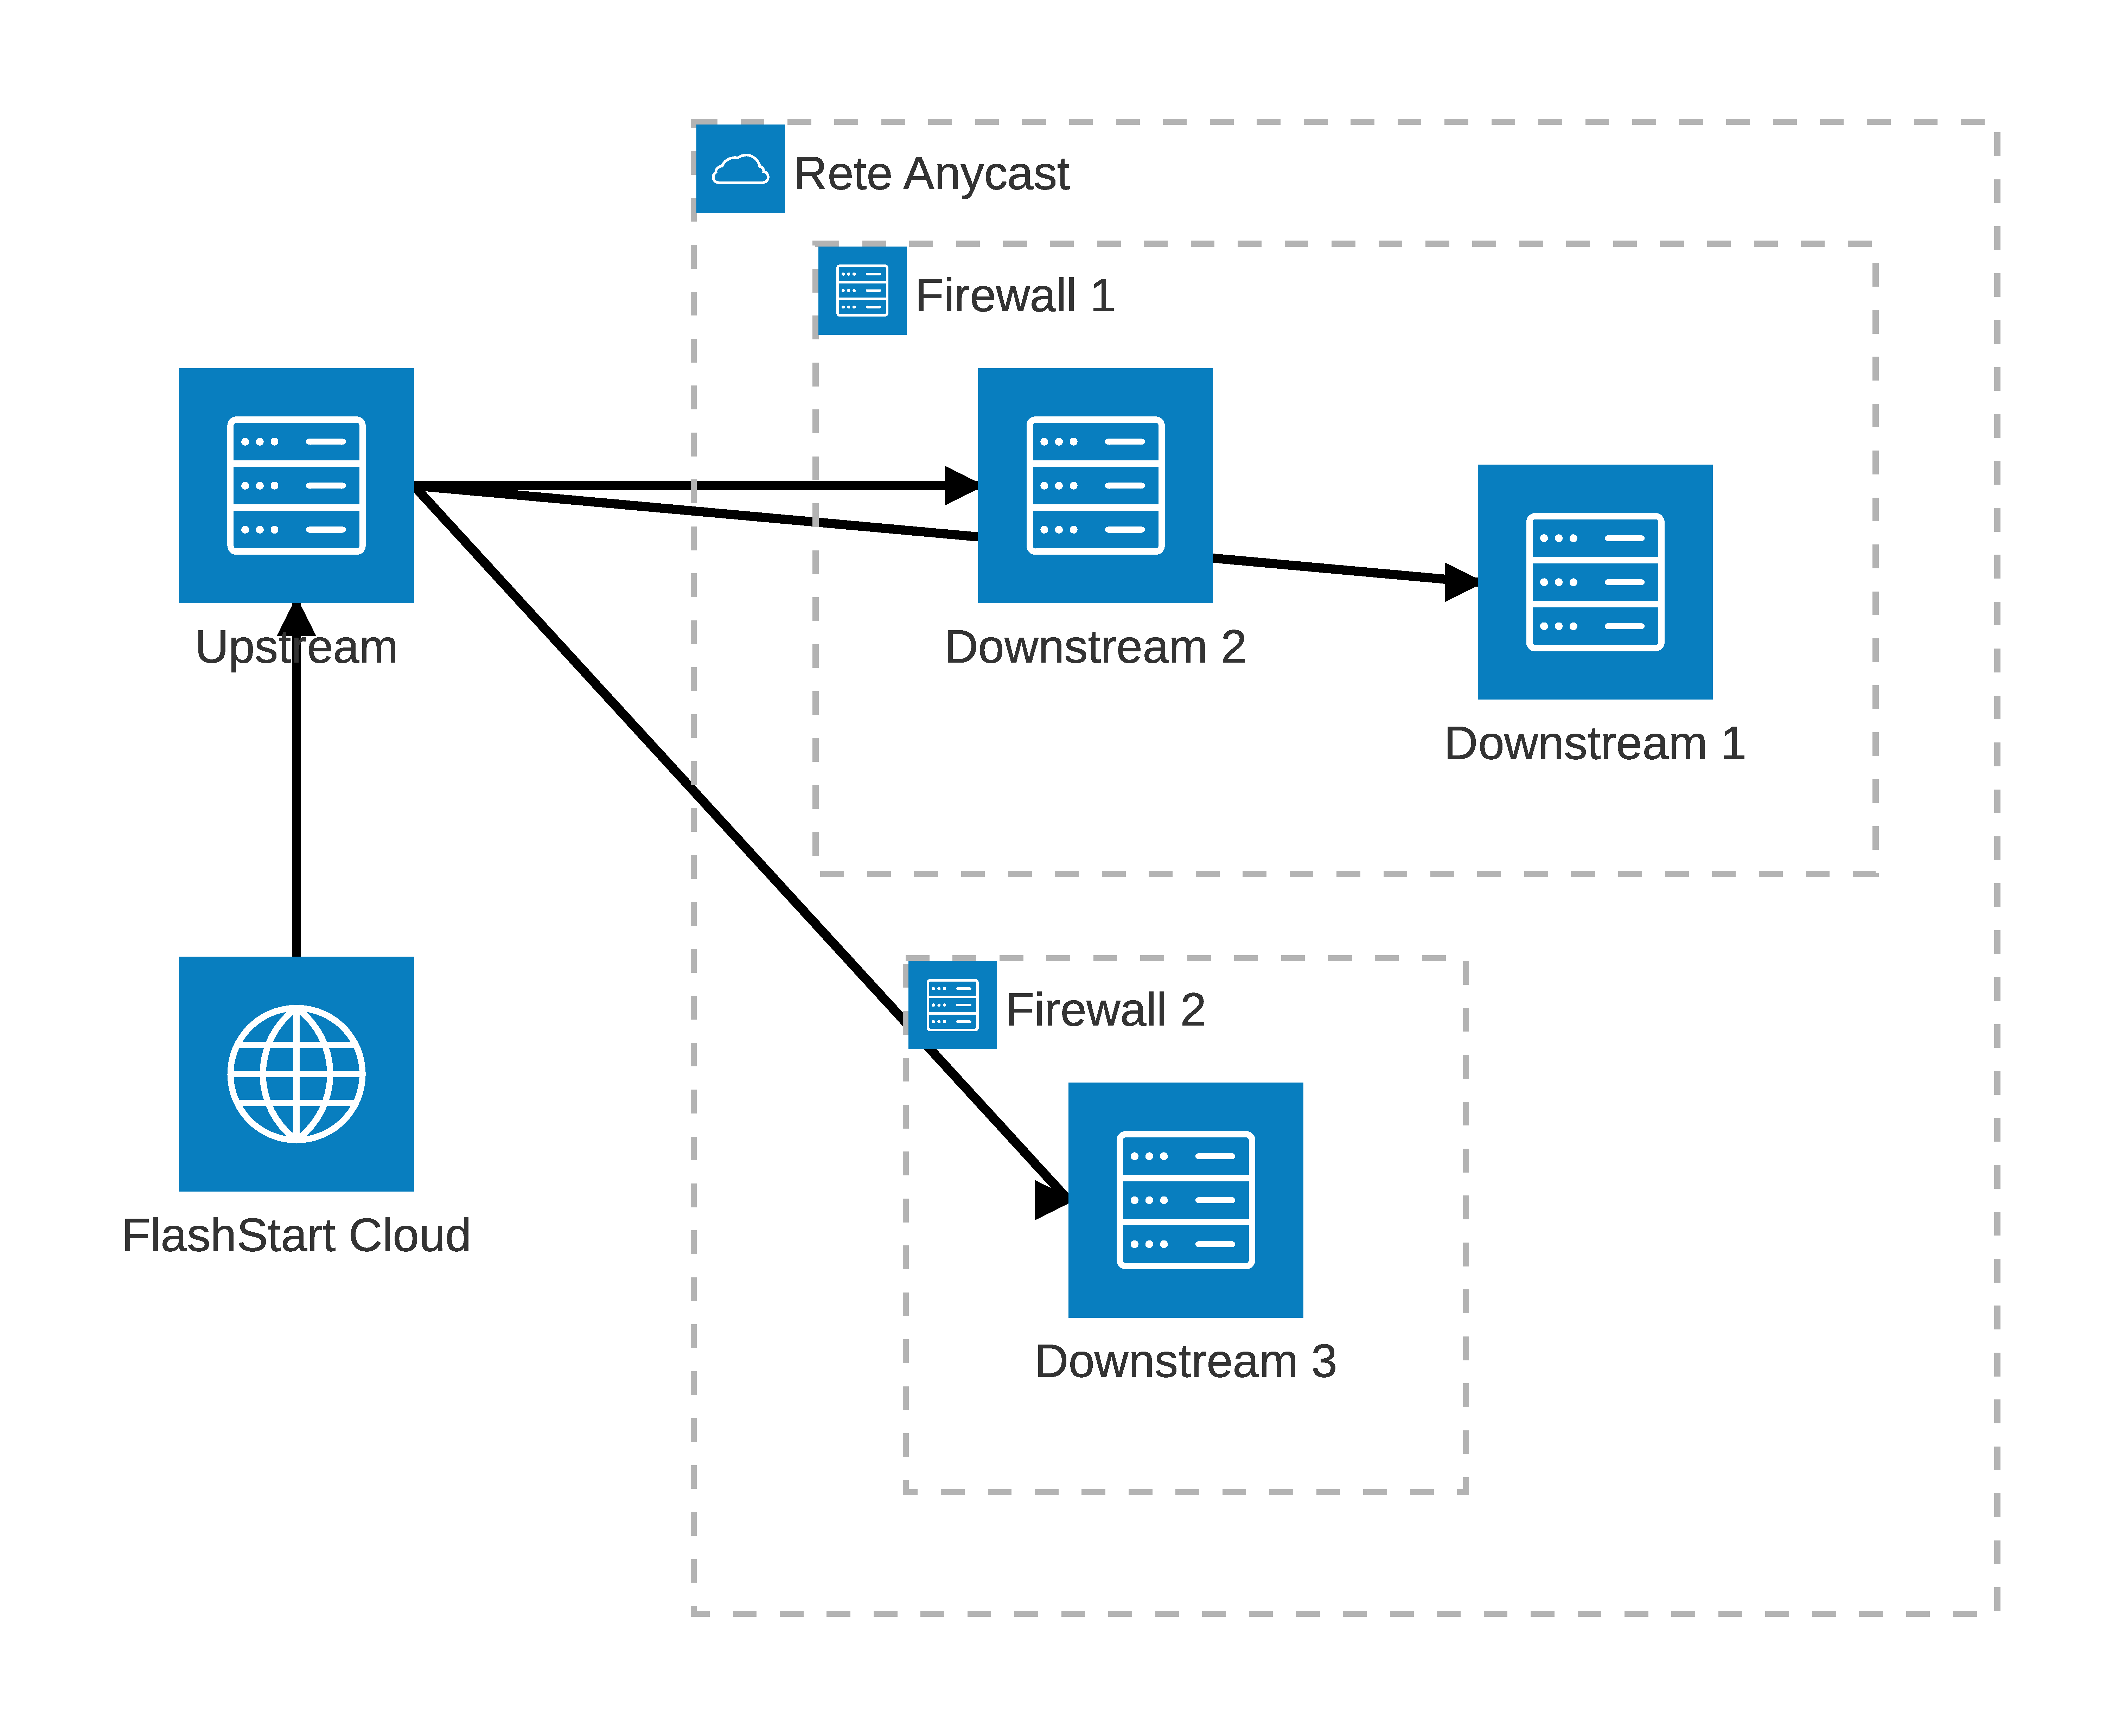
\includegraphics[width=.6\linewidth]{figures/legacy-architecture.pdf}
    \caption{Architettura del servizio legacy}
    \label{fig:legacy-architecture}
\end{figure}
\chapter{Analisi}
\label{chapter:analysis}
In questo capitolo vengono evidenziati i requisiti del progetto, analizzando i limiti imposti dalla quantità di risorse a disposizione da ciascun server all'interno della rete.

\section{Obbiettivi}
L'obbiettivo del progetto è quello di riscrivere il servizio di diagnostica della latenza, partendo da un codice monolitico scritto in php e python.
La struttura di comunicazione deve rimanere quella attuale mantenendo le tre componenti descritte in precedenza.


%----------------------------------------------------------------------------------------
% BIBLIOGRAPHY
%----------------------------------------------------------------------------------------

\backmatter

\nocite{*} % Remove this as soon as you have the first citation

\bibliographystyle{alpha}
\bibliography{bibliography}

\begin{acknowledgements} % this is optional
Optional. Max 1 page.
\end{acknowledgements}

\end{document}
